% ==========================================
% NUOVO ARGOMENTO: SORGENTI E PROCESSI
% ==========================================

\section{Modellizzazione delle Sorgenti di Informazione}

Fino a questo momento abbiamo calcolato l'entropia di singole variabili o di coppie isolate. Tuttavia, in uno scenario di telecomunicazioni reale, un trasmettitore non emette un solo simbolo per poi spegnersi, ma genera un flusso continuo di dati nel tempo. 

Una generica sorgente di informazione è modellabile matematicamente come un generatore che produce una sequenza temporale di variabili aleatorie $\{X_i\}_{i \in \mathbb{Z}}$. Questa sequenza prende il nome di \textbf{processo aleatorio tempo-discreto}.

\begin{center}
\vspace{0.3cm}
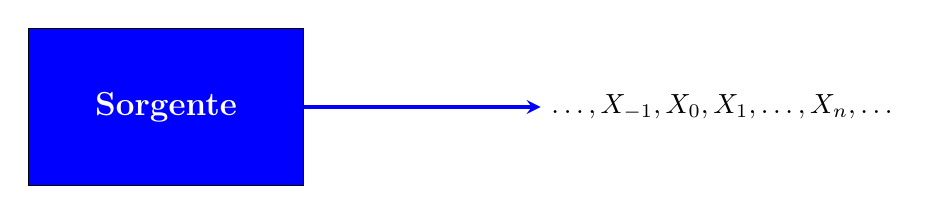
\begin{tikzpicture}[>=stealth]
    % Blocco Sorgente
    \node[draw, fill=blue, text=white, minimum width=3.5cm, minimum height=2cm, font=\large\bfseries] (source) {Sorgente};
    % Freccia in uscita
    \draw[->, blue, very thick] (source.east) -- +(3,0) node[right, text=black, font=\normalsize] {$\dots, X_{-1}, X_0, X_1, \dots, X_n, \dots$};
\end{tikzpicture}
\vspace{0.3cm}
\end{center}

\subsection{Ipotesi Semplificative del Modello}

Assumeremo che il processo generato dalla sorgente rispetti tre ipotesi fondamentali:
\begin{enumerate}
    \item \textbf{Ampiezza discreta:} L'alfabeto $\mathcal{X}$ da cui vengono estratti i simboli ha cardinalità finita (es. codice binario, alfabeto testuale).
    \item \textbf{Stazionarietà in senso stretto (di ordine qualsiasi):} Le leggi statistiche che governano la sorgente non cambiano col passare del tempo. La probabilità di osservare una certa sequenza oggi è identica alla probabilità di osservarla domani.
    \item \textbf{Caratterizzazione completa:} Si assume che tutte le PMF (Probability Mass Function) congiunte di qualsiasi ordine siano note a priori all'analista.
\end{enumerate}

\subsection{Sorgenti Senza Memoria (DMS)}

All'interno della famiglia dei processi stazionari, esiste una sottoclasse di fondamentale importanza teorica. 
Una sorgente si dice \textbf{senza memoria} se i simboli emessi sono tra loro \textit{statisticamente indipendenti}. In altre parole, il simbolo $X_k$ che la sorgente sta per emettere non è in alcun modo influenzato dalla conoscenza dei simboli $X_{k-1}, X_{k-2}$ emessi in precedenza. 

L'acronimo \textbf{DMS} (\textit{Discrete Memoryless Source}).

\subsection{Contenuto Informativo di una DMS (Entropia di Blocco)}

Vogliamo ora calcolare quanta informazione è contenuta in un intero blocco di simboli consecutivi emessi da una DMS. 
Consideriamo un blocco di lunghezza $n$, che possiamo indicare come un vettore aleatorio: $\mathbf{X}^n = (X_1, X_2, \dots, X_n) \in \mathcal{X}^n$.

Applicando per generalizzazione la definizione di entropia congiunta vista nel capitolo precedente, l'entropia del blocco è il valore atteso del logaritmo dell'inverso della PMF congiunta di ordine $n$:
\begin{equation}
    H(\mathbf{X}^n) = H(X_1, X_2, \dots, X_n) = \sum_{\mathbf{x}^n \in \mathcal{X}^n} p_{\mathbf{X}^n}(\mathbf{x}^n) \log \left[ \frac{1}{p_{\mathbf{X}^n}(\mathbf{x}^n)} \right]
\end{equation}

Sviluppiamo matematicamente questa espressione sfruttando la definizione di DMS. Poiché la sorgente è \textit{senza memoria}, le variabili sono indipendenti. Di conseguenza, la probabilità congiunta di osservare l'intero blocco è semplicemente il prodotto delle probabilità marginali dei singoli simboli:
\begin{equation}
    p_{\mathbf{X}^n}(\mathbf{x}^n) = \prod_{i=1}^{n} p_{X_i}(x_i)
\end{equation}

Sostituendo questo prodotto all'interno del calcolo del valore atteso (Entropia) e sfruttando le proprietà dei logaritmi, i passaggi si svolgono come segue:
\begin{align}
    H(\mathbf{X}^n) &= \mathbb{E} \left[ \log \frac{1}{\prod_{i=1}^{n} p_{X_i}(X_i)} \right] \nonumber \\
                    &= \mathbb{E} \left[ \sum_{i=1}^{n} \log \frac{1}{p_{X_i}(X_i)} \right] \nonumber \\
                    &= \sum_{i=1}^{n} \mathbb{E} \left[ \log \frac{1}{p_{X_i}(X_i)} \right] \nonumber \\
                    &= \sum_{i=1}^{n} H(X_i)
\end{align}

Infine, ricordiamo che la sorgente è \textit{stazionaria}, il che significa che l'entropia marginale di ogni singolo istante di tempo è costante e identica a quella del primo simbolo ($H(X_i) = H(X_1)$ per ogni $i$). La somma di $n$ termini identici ci porta al risultato finale:
\begin{equation}
    \boxed{ H(\mathbf{X}^n) = n \cdot H(X_1) }
\end{equation}
L'entropia di un blocco di $n$ simboli generati da una sorgente senza memoria è esattamente $n$ volte l'entropia di un singolo simbolo.

\subsection{Il Tasso Entropico (Entropy Rate)}

Per valutare il flusso di informazione di un processo in modo indipendente dalla lunghezza specifica del blocco $n$ che stiamo analizzando, si introduce una metrica asintotica chiamata \textbf{Tasso Entropico} (o \textit{Entropy Rate}). 

Esso è definito come il limite per $n$ che tende all'infinito della quantità media di informazione trasportata da un singolo simbolo all'interno di un blocco infinito:
\begin{equation}
    H_\infty(\mathcal{X}) = \lim_{n \to \infty} \frac{H(\mathbf{X}^n)}{n}
\end{equation}

Sostituendo il risultato ottenuto nel paragrafo precedente per le DMS ($H(\mathbf{X}^n) = n H(X_1)$), il limite diventa banale:
\begin{equation}
    H_\infty(\mathcal{X}) = \lim_{n \to \infty} \frac{n \cdot H(X_1)}{n} = H(X_1)
\end{equation}

\textbf{Conclusione fisica:} Per una sorgente Discreta Senza Memoria, il tasso entropico coincide esattamente con l'entropia della singola emissione marginale. In termini pratici, questo significa che in una DMS non c'è "ridondanza nascosta" tra un simbolo e l'altro; osservare blocchi di dati molto lunghi non ci aiuterà a comprimere i dati meglio di quanto potremmo fare comprimendo simbolo per simbolo, poiché ogni nuova emissione porta con sé una quantità di incertezza "fresca" e totalmente indipendente dal passato.

% ==========================================
% NUOVO ARGOMENTO: SORGENTI CON MEMORIA
% ==========================================

\section{Sorgenti con Memoria}

Rimuoviamo ora l'ipotesi forte di indipendenza tra i simboli (DMS), conservando unicamente l'ipotesi di stazionarietà. In una \textbf{sorgente con memoria}, la probabilità che venga emesso un certo simbolo dipende dai simboli che lo hanno preceduto nel tempo. Esempi classici sono il linguaggio umano (la probabilità che la lettera 'U' segua la lettera 'Q' è altissima) o il meteo.

Per modellare questa situazione, ricordiamo la \textbf{Legge di Bayes} generalizzata a $n$ variabili (nota come regola della catena per le probabilità). La probabilità congiunta di osservare un'intera sequenza $\mathbf{x}^n$ si può fattorizzare condizionando ogni simbolo al suo intero passato:
\begin{equation}
    p_{\mathbf{X}^n}(\mathbf{x}^n) = p_{X_1}(x_1) \cdot p_{X_2|X_1}(x_2|x_1) \cdot p_{X_3|X_2,X_1}(x_3|x_2,x_1) \dots p_{X_n|X_{n-1},\dots,X_1}(x_n|x_{n-1},\dots,x_1)
\end{equation}

Di conseguenza, applicando lo stesso principio logico esplorato con le coppie di variabili aleatorie, l'entropia congiunta dell'intero blocco di dati $\mathbf{X}^n$ si espande in una somma di entropie condizionate:
\begin{equation}
    H(\mathbf{X}^n) = H(X_1) + H(X_2|X_1) + \dots + H(X_n|X_{n-1}, \dots, X_1)
\end{equation}
Che possiamo riscrivere in forma compatta con una sommatoria:
\begin{equation}
    H(\mathbf{X}^n) = \sum_{i=1}^{n} H(X_i | X_{i-1}, \dots, X_1)
\end{equation}

\subsection{Il Concetto di Innovazione}

Soffermiamoci sul generico termine della sommatoria, definendolo esplicitamente tramite il valore atteso:
\begin{equation}
    H(X_i | X_{i-1}, \dots, X_1) = \sum_{\mathbf{x}^i \in \mathcal{X}^i} p_{\mathbf{X}^i}(\mathbf{x}^i) \log \left( \frac{1}{p_{X_i | X_{i-1}, \dots, X_1}(x_i | x_{i-1}, \dots, x_1)} \right)
\end{equation}

Questa quantità ha un significato fisico e informatico profondissimo: rappresenta \textbf{l'incertezza residua sul simbolo $X_i$ una volta che tutti i simboli precedenti sono noti}. 
In altre parole, rappresenta quella parte di informazione trasportata dall'$i$-esimo simbolo che \textit{non era assolutamente predicibile} guardando al passato. Nella teoria dei segnali, questa quantità di informazione "fresca" o "nuova" prende il nome di \textbf{Innovazione}.

\section{Tasso Entropico di Sorgenti con Memoria}

Vogliamo ora calcolare il tasso entropico $H_\infty(\mathcal{X})$ per questa sorgente, ovvero l'incertezza media per simbolo valutata su una sequenza di lunghezza infinita:
\begin{equation}
    H_\infty(\mathcal{X}) = \lim_{n \to \infty} \frac{H(\mathbf{X}^n)}{n} 
\end{equation}

Sostituendo l'entropia di blocco con la sommatoria appena ricavata tramite la regola della catena, otteniamo:
\begin{equation}
\label{eq:rate_sum}
    H_\infty(\mathcal{X}) = \lim_{n \to \infty} \frac{1}{n} \sum_{i=1}^{n} H(X_i | X_{i-1}, \dots, X_1)
\end{equation}

Dal punto di vista analitico, abbiamo il limite di una media aritmetica di termini. Per risolvere questa operazione in modo elegante, ricorriamo a uno strumento dell'analisi matematica: il Teorema della media di Cesàro.

\subsection{Il Teorema di Cesàro}

Il teorema stabilisce che se abbiamo una successione numerica $\{b_n\}$ che converge a un limite ben preciso $b$, allora anche la successione formata dalle sue \textit{medie aritmetiche} convergerà allo stesso identico limite $b$.
\begin{equation*}
    \lim_{n \to \infty} b_n = b \implies \lim_{n \to \infty} \frac{1}{n} \sum_{i=1}^{n} b_i = b
\end{equation*}

\subsubsection{Applicazione al Tasso Entropico}
Rinominiamo i nostri complessi termini di entropia condizionata per adattarli al teorema. Sia $b_n$ l'incertezza del singolo $n$-esimo simbolo dato tutto il suo passato:
\begin{equation}
    b_n = H(X_n | X_{n-1}, \dots, X_1)
\end{equation}
Il teorema di Cesàro ci garantisce che, se l'incertezza dell'$n$-esimo simbolo (conoscendo il passato) tende a stabilizzarsi verso un limite, allora anche il tasso entropico globale tenderà a quel limite. 
Questo ci permette di semplificare drasticamente i calcoli: \textit{invece di calcolare il limite della media di tutte le entropie, possiamo semplicemente calcolare il limite dell'ultima entropia condizionata}.
\begin{equation}
    \boxed{ H_\infty(\mathcal{X}) = \lim_{n \to \infty} H(X_n | X_{n-1}, \dots, X_1) }
\end{equation}

% ==========================================
% NUOVO ARGOMENTO: COMPRESSIONE A BLOCCHI
% ==========================================

\section{Compressione di Sorgenti con Memoria: L'Approccio a Blocchi}

Riprendiamo la definizione formale di processo aleatorio: una sequenza temporale infinita di variabili aleatorie $\{\dots, X_{-1}, X_0, X_1, \dots\}$. In ogni istante discreto $t$, la sorgente emette un simbolo rappresentato dalla variabile $X_t$.

Come abbiamo visto, in una sorgente con memoria l'estrazione della variabile $X_t$ non è indipendente, ma è fortemente influenzata da ciò che è stato emesso prima. 
Per rendere il problema trattabile matematicamente, introduciamo l'ipotesi di \textbf{Stazionarietà Stretta}. Ipotizziamo cioè che le proprietà statistiche (le leggi di probabilità) del processo non cambino con il passare del tempo. 

Formalmente, un processo è strettamente stazionario se, per qualsiasi lunghezza $k$ e per qualsiasi traslazione temporale $h$, la probabilità congiunta rimane invariata:
\begin{equation}
    \mathbb{P}\{X_1 = x_{i_1}, \dots, X_k = x_{i_k}\} = \mathbb{P}\{X_{1+h} = x_{i_1}, \dots, X_{k+h} = x_{i_k}\}
\end{equation}
In parole povere: la probabilità di osservare la sequenza "C-I-A-O" oggi è identica alla probabilità di osservare la sequenza "C-I-A-O" tra un mese.

\subsection{Il Problema Ingegneristico della Memoria}

Se volessimo comprimere in modo perfettamente ottimo questa sorgente, dovremmo applicare un codice (es. Huffman) tenendo conto dell'entropia condizionata. Ma c'è un ostacolo insormontabile:
\begin{quote}
    \textbf{Problema Pratico:} Codificare il simbolo corrente tenendo traccia e calcolando le probabilità condizionate basate su \textit{tutta l'infinita storia passata} della sorgente è computazionalmente impossibile e richiederebbe una memoria infinita.
\end{quote}

\subsection{La Soluzione: Macrosimboli e Codifica di Blocco}

Per aggirare questo ostacolo, l'ingegneria dell'informazione adotta una strategia di raggruppamento. Invece di codificare un singolo simbolo alla volta guardando al suo passato, \textbf{raggruppiamo il flusso continuo di simboli in blocchi finiti di lunghezza $n$}.

Questo approccio trasforma radicalmente la prospettiva del problema:
\begin{enumerate}
    \item Un intero blocco di $n$ simboli consecutivi (una "parola" di lunghezza $n$) viene ora considerato e trattato dal codificatore come un singolo \textbf{Macrosimbolo}.
    \item Se l'alfabeto originale di partenza era $\mathcal{X}$ (con cardinalità $|\mathcal{X}|$), il nuovo macrosimbolo apparterrà a un \textbf{nuovo alfabeto esteso} denominato $\mathcal{X}^n$.
    \item La cardinalità di questo nuovo alfabeto cresce esponenzialmente. Il numero totale di possibili macrosimboli distinti che il codificatore dovrà gestire sarà pari a $|\mathcal{X}|^n$.
\end{enumerate}

\subsubsection*{Esempio Intuitivo}
Se la nostra sorgente originale emette bit ($\mathcal{X} = \{0, 1\}$, cardinalità $2$) e noi decidiamo di usare blocchi di lunghezza $n=8$ (i Byte), il nostro codificatore non vedrà più i singoli bit, ma vedrà una sequenza di Macrosimboli estratti dal nuovo alfabeto $\mathcal{X}^8$, che contiene $2^8 = 256$ "parole" diverse (da \texttt{00000000} a \texttt{11111111}).

\subsubsection*{Il Vantaggio della Codifica a Blocchi}
Raggruppando i simboli in blocchi sufficientemente lunghi, la dipendenza statistica (la memoria) \textit{all'interno} del blocco viene catturata dalla probabilità congiunta del macrosimbolo stesso. 
In questo modo, ci riduciamo a una condizione in cui \textbf{occorre codificare un singolo macrosimbolo alla volta}. Se $n$ è abbastanza grande, la dipendenza tra un macrosimbolo e il successivo diventa trascurabile, permettendoci di applicare gli algoritmi classici (come Shannon o Huffman) sul nuovo alfabeto $\mathcal{X}^n$ quasi come se stessimo lavorando con una sorgente senza memoria (DMS), avvicinandoci così al tasso entropico teorico $H_\infty(\mathcal{X})$.

\section{Limiti di Comprimibilità: Il Teorema Fondamentale}

Ora che abbiamo definito il concetto di Macrosimbolo (il blocco di $n$ simboli), applichiamo la teoria della codifica sorgente a questo nuovo alfabeto $\mathcal{X}^n$.

Sappiamo che qualsiasi codice, per essere univocamente decifrabile, deve rispettare la Disuguaglianza di Kraft. Da questa, abbiamo derivato il \textbf{Primo Teorema di Shannon}, il quale garantisce l'esistenza di un codice a prefisso la cui lunghezza media $L$ rispetta il vincolo: $H(Y) \le L < H(Y) + 1$.

\subsection{Dalla Codifica del Blocco al Costo per Simbolo}

Applichiamo la relazione di Shannon al nostro vettore aleatorio $\mathbf{X}^n = (X_1, \dots, X_n)$. 
Sia $L_{blocco}$ il numero medio di bit necessari per codificare \textit{l'intero macrosimbolo} di lunghezza $n$. Avremo:
\begin{equation}
    H(\mathbf{X}^n) \le L_{blocco} < H(\mathbf{X}^n) + 1
\end{equation}

Tuttavia, a livello ingegneristico, non ci interessa tanto quanto costa il macrosimbolo, ma \textbf{qual è il costo medio per ogni singolo simbolo originario}. Per trovare questo valore, definiamo la lunghezza media per simbolo $L_n = \frac{L_{blocco}}{n}$ e dividiamo tutta la disuguaglianza per $n$:
\begin{equation}
    \frac{H(\mathbf{X}^n)}{n} \le \frac{L_{blocco}}{n} < \frac{H(\mathbf{X}^n)}{n} + \frac{1}{n}
\end{equation}
\begin{equation}
    \frac{H(\mathbf{X}^n)}{n} \le L_n < \frac{H(\mathbf{X}^n)}{n} + \frac{1}{n}
\end{equation}

\subsection{Il Limite Asintotico e il Tasso Entropico}

Cosa succede se raggruppiamo i dati in blocchi sempre più grandi? Studiamo il comportamento asintotico facendo tendere la lunghezza del blocco all'infinito ($n \to \infty$). 
Ricordando la definizione di Tasso Entropico $H_\infty(\mathcal{X}) = \lim_{n \to \infty} \frac{H(\mathbf{X}^n)}{n}$, la disequazione diventa:
\begin{equation}
    H_\infty(\mathcal{X}) \le \lim_{n \to \infty} L_n < H_\infty(\mathcal{X}) + \lim_{n \to \infty} \frac{1}{n}
\end{equation}

Poiché il termine $\frac{1}{n}$ tende inesorabilmente a $0$ (diventando una quantità arbitrariamente piccola $\epsilon$), otteniamo il teorema fondamentale della codifica per sorgenti con memoria:
\begin{equation}
\boxed{ H_\infty(\mathcal{X}) \le L_n < H_\infty(\mathcal{X}) + \epsilon }
\end{equation}

Questo risultato è straordinario: ci dice che, mediante la codifica a blocchi, se prendiamo blocchi sufficientemente lunghi, possiamo arrivare ad utilizzare un numero medio di bit per simbolo \textbf{vicino quanto vogliamo al tasso entropico della sorgente}.

\section{Conseguenze: Perché la memoria è un vantaggio?}

Analizziamo ora le conseguenze pratiche di questa scoperta, confrontando le sorgenti senza memoria (DMS) con le sorgenti con memoria.

\subsubsection*{Caso 1: Sorgenti Senza Memoria (DMS)}
Abbiamo dimostrato in precedenza che per una sorgente con simboli indipendenti l'entropia del blocco è la somma delle entropie marginali: $H(\mathbf{X}^n) = nH(X_1)$. Sostituendo nella formula precedente, il limite si semplifica:
\begin{equation}
    H(X) \le L_n < H(X) + \epsilon
\end{equation}
Per le DMS, il tasso entropico \textit{coincide} con l'entropia del singolo simbolo. Raggruppare i dati in blocchi non abbassa il limite teorico invalicabile, serve unicamente a ridurre quello "spreco" di $\approx 1$ bit dovuto all'arrotondamento del Codice di Shannon.

\subsubsection*{Caso 2: Sorgenti Con Memoria}
Ricordiamo la definizione di tasso entropico per sorgenti con memoria tramite il limite di Cesàro:
\begin{equation}
    H_\infty(\mathcal{X}) = \lim_{n \to \infty} H(X_n | X_{n-1}, \dots, X_1)
\end{equation}
Sappiamo anche, dal teorema basato sulla Mutua Informazione, che \textbf{il condizionamento non aumenta mai l'entropia} (anzi, in presenza di dipendenza statistica, la fa diminuire strettamente):
\begin{equation}
    H(X_n | X_{n-1}, \dots, X_1) \le H(X_n)
\end{equation}

Di conseguenza, per una sorgente con memoria è matematicamente garantito che il tasso entropico sia inferiore all'entropia del singolo simbolo:
\begin{equation}
    \mathbf{H_\infty(\mathcal{X}) \le H(X)}
\end{equation}

\begin{quote}
    \textbf{Regola d'oro dell'informazione:} \\
    \textit{"La memoria è struttura, e la struttura significa prevedibilità."}
\end{quote}

Le sorgenti con memoria godono di limiti di comprimibilità molto più significativi (molto più bassi) rispetto alle sorgenti senza memoria. Se ignoro la memoria e comprimo simbolo per simbolo, mi fermerò al muro dell'entropia marginale $H(X)$. Ma se raggruppo i dati, sfrutto le dipendenze statistiche: il fatto che un evento sia probabile conoscendo il passato abbassa la sua quantità di informazione (innovazione), permettendomi di usare meno bit. Più la sorgente è strutturata, più posso spingere la compressione verso il limite inferiore assoluto $H_\infty(\mathcal{X})$.